%%!TeX program = xelatex
%% 부득이하게 pdflatex을 사용해야 할 경우 위의 magic comment를 제거하십시오.

% Initiated by 정민석(2014년도 경기과학고 수학과전문교원)
% Continously being modified by 경기과학고 TeX 사용자협회
% Website : http://latex.gs.hs.kr
% 박기현(선생님)과 한수민(37기) 학생이 본문 나누어진 버전으로 개선함.
% 채상미(선생님)과 권준우(37기) 학생이 2021년 최종 수정.
\documentclass{gshs_report}
% 아래의 함수를 사용하면 이미지 파일들을 같은 디렉토리 내에 images 라는 이름을 가진 폴더를 생성한 후, 그 폴더 안에 넣어 사용할 수 있습니다.
% 사용하고자 한다면 주석을 푸십시오.
\graphicspath{{images/}}
% 이곳에 필요한 별도의 패키지들을 적어넣으시오.
%\usepackage{...}
\usepackage{verbatim} % for commment, verbatim environment
\usepackage{spverbatim} % automatic linebreak verbatim environment
%\usepacakge{indentfirst}
\usepackage{tikz}
%\tikzset{
%	image label/.style={
%		every node/.style={
			%fill=black,
			%text=white,
%			font=\sffamily\scriptsize,
%			anchor=south west,
%			xshift=0,
%			yshift=0,
%			at={(0,0)}
%		}
%	}
%}
\usepackage{amsmath}
\usepackage{amsfonts}
\usepackage{amssymb}
\usepackage{float}
\usepackage{graphicx}
\usepackage{tabularx}
\usepackage{multirow}
\usepackage{booktabs}
\usepackage{longtable}
\usepackage{gensymb}
\usepackage{wrapfig}
% \usepackage{hyperref}
% \hypersetup{
%     colorlinks=true,
%     allcolors=blue,
%     linkcolor=blue,
%     filecolor=magenta,      
%     urlcolor=cyan,
% }

%\usepackage{subcaption}
%\usepackage{floatrow}
%\usepackage{pict2e}
%\usepackage[backend=biber,style=authoryear]{biblatex}
%\usepackage{biblatex}
\usepackage{pgfplots}
\pgfplotsset{
	compat=newest,
	label style={font=\sffamily\scriptsize},
	ticklabel style={font=\sffamily\scriptsize},
	legend style={font=\sffamily\tiny},
	major tick length=0.1cm,
	minor tick length=0.05cm,
	every x tick/.style={black},
}

\usetikzlibrary{shapes}
\usetikzlibrary{plotmarks}
\usepackage{listings}
\usepackage{hologo}
\usepackage{makecell}
\usepackage{color}
\lstset{
	basicstyle=\small\ttfamily,
	columns=flexible,
	breaklines=true
}

\citation
\bibdata

%: ----------------------------------------------------------------------
%:               보고서 정보를 입력하시오
% ----------------------------------------------------------------------
% 아래와 같은 command를 만들면 길이가 긴 용어를 간편하게 사용할 수 있습니다. 단, 이미 지정된 함수명들은 새로운 함수명으로 사용할 수 없습니다.
% 연, 월, 일은 보고서 제출 날짜에 맞게 수정하십시오.

\newcommand{\gshs}{Gyeonggi Science High School for the Gifted }

% \researchtype{기초} % 기초 / 심화
% \reporttype{중간/결과} % 중간 / 결과

\title{정보 엔트로피를 이용한 여러 조건에서의 \linebreak 최적의 확률 분포 계산 및 해석}

% \title{제목} % 제목 개행 시 \linebreak 사용. \\나 \newline 은 안됨.
% \englishtitle{English Title}% 제목 개행 시 \linebreak 사용. \\나 \newline 은 안됨.

\author[1] {21032 김희윤}
% \email[1]{}
\author[2] {21033 남도현}
% \email[2]{}
\author[3] {21052 배요한}
% \email[3]{}
% \email[1]{(author@email.address)} % 제 1 저자 이메일
% \author[2] {} % 제 2 저자명
% \email[2]{} % 제 2 저자 이메일
% \advisor{Teacher} % 지도교사명
% \advisorEmail{(teacher@email.address)} % 지도교사 이메일

%%%%%%%%%%%%%%%%%%%%%%%%%%%%%%%%%%%%%%%%%%%%%%%
%%%% researchtype이 '심화'일 경우에만 나타남 %%%%
% \professor{Professor} % 지도교수명
% \professorEmail{(professor@email.address)} % 지도교수 이메일
% %%%%%%%%%%%%%%%%%%%%%%%%%%%%%%%%%%%%%%%%%%%%%%%%
% \summitdate{2020}{01}{01} % 제출일 (연, 월, 일)
% \newtheorem{definition}{정의}
 % usepackage 등의 명령어는 여기에.

% \begin{center}
%     \Large
%     \textbf{정보 엔트로피를 이용한 여러 조건에서의 확률 분포 계산 및 해석}
        
%     \vspace{0.4cm}
%     \large
%     Thesis Subtitle
        
%     \vspace{0.4cm}
%     \textbf{Author Name}
       
%     \vspace{0.9cm}
%     \textbf{Abstract}
% \end{center}

\usepackage{cite}
\usepackage{textcomp}
\usepackage{tocloft}
\setlength{\cftbeforesecskip}{0pt}
\setlength{\cftbeforesubsecskip}{0pt}
\setlength{\cftbeforesubsubsecskip}{0pt}
% 본문 시작
\begin{document}
        \makecover
	%표지만들기
	%makecover 함수와 관련하여 "Underfull \hbox (badness 10000) in paragraph" 오류는 무시하십시오. (TeXstudio ver 2.9.4 오류 기준)
	%\makecover
	

	%\baselineskip=2.2em         % line spacing in the paragraph
	% \maketitle

\begin{abstractskor}
	% \addcontentsline{toc}{section}{초록}  %%% TOC에 표시
	\noindent{
		본 보고서는 정보 엔트로피에 대한 탐구로 여러 제약 조건이 걸려있는 경우의 정보 엔트로피를 최대화시키는 확률 분포를 이론적으로 탐색하고 시뮬레이션을 통해 이를 검증하는 것을 목표로 한다. 정보 엔트로피는 통계역학에서 특정 사건이 생길 수 있는 평균적인 로그확률로 계산된다. 이는 열역학적으로 정의된 두 엔트로피와 상통하며 열역학 제 2법칙에서도 볼 수 있듯이 계는 항상 엔트로피가 최대인 상태를 점유한다. 이는 엔트로피가 최대인 상황을 점유할 확률이 높다는 것으로 정보 엔트로피의 경우 주어진 조건에 대해서 평균 정보량이 최대인 조건을 탐색한다는 의미이다.
        제약조건은 총 확률의 합이 1, 기댓값이 주어진 경우, 표준편차가 주어진 경우로 3가지가 있으며 라그랑주 승수법을 이용하여 확률분포가 취해야 할 조건을 구한다. 총 확률이 1인 경우에는 균일 분포가 최대였으며 기댓값이 주어진 경우에는 볼츠만 분포, 표준편차가 주어진 경우에는 정규 분포가 최대였다. 이는 연속 확장을 할 경우 관련 상수를 쉽게 찾을 수 있으나 이산 확률 분포로 취급하는 순간 관련 상수를 찾기 어려웠으며 시뮬레이션을 통해 주어진 원리와 상통하는지 확인하였다.
        시뮬레이션 기법은 최적화 기법 중 하나인 유전 알고리즘이다. $n=20$인 상황에 대해서 $p_1, p_2, \cdots p_n$을 유전자로 취급하며 관련 연산을 정의하고 $H(p)$가 최대인 분포를 탐색하였다. 그 결과는 이론 분석한 결과와 일치하였으며 kullback-leibler divergence를 이용하여 차이를 비교하였다.

	}
\end{abstractskor}






 % Abstract
	
	%%%%%%%%%%%%%%%%%%%%%%%%%%%%%%%%%%%%%%%%%%%%%%%%%%%%%%%%%%%
	%%%% Main Document %%%%%%%%%%%%%%%%%%%%%%%%%%%%%%%%%%%%%%%%
	%%%%%%%%%%%%%%%%%%%%%%%%%%%%%%%%%%%%%%%%%%%%%%%%%%%%%%%%%%%
	% \cleardoublepage
	% \clearpage
	\renewcommand{\thepage}{\arabic{page}}
	\setcounter{page}{1}
	
	%각 장을 아래와 같이 sub 폴더 안에 만들어서 넣으면 편리하다.
	\section{서론}

엔트로피란 흔히 '무질서도'라고 알려진 개념이다. 정확한 정의로는 열역학적으로 사용이 불가능한 에너지를 나타내는 상태 함수이다. 열역학 제 2법칙과 관련된 물리량으로 크게 열역학적 정의, 통계역학적 정의, 정보이론의 정의로 나뉜다.

열역학적 정의는 클라우지우스가 카르노 기관에 대해 탐구하며 정의하였다.
\begin{equation}
    dS = \frac{dQ}{T}
\end{equation}
통계역학에서 사용되는 엔트로피는 볼츠만이 정의하였으며 기체 입자 계 (ensemble)에서 특정 상태가 일어날 경우의 수 $\Omega$에 로그를 취한 값을 갖는다.
\begin{equation}
    S = k_{B} \ln{\Omega}
\end{equation}

이를 토대로 섀넌이 정보 엔트로피 또는 섀넌 엔트로피(Shannon Entropy)를 특정 사건이 생길 수 있는 평균적인 로그 확률로 정의하였다. 거시 상태를 점유하는 미시 상태의 수를 상대적인 확률로 취급한 것이며 깁스의 entropy formula에 의해 매개된다. 즉, 미지의 정보가 많아 확실성이 떨어지는 상태가 정보 엔트로피가 높은 상태가 된다. 결론적으로 세 엔트로피의 정의는 동일하다.

최대 엔트로피 원리란 시스템의 현재 지식 상태를 가장 잘 나타내는 확률 분포는 가장 큰 엔트로피를 갖는 확률 분포라는 것이다. 초기 상태에 대한 정보가 부족한 경우 모든 상태를 균일하게 탐색할 필요성이 있으며 그러한 확률 분포는 엔트로피가 최대가 되는 확률 분포와 같다. 이는 열역학 제 2법칙과도 연관이 있다.

본 연구에서는 특정 조건에서 엔트로피가 최대가 되는 확률 분포에 대한 탐색을 두 가지 방법으로 진행하였다. 첫 번째 방법은 라그랑주 승수법을 이용하여 확률 분포를 이론적으로 계산해 내었다. 두 번째 방법으로는 최적화 문제에 흔히 쓰이는 유전 알고리즘(Genetic Algorithm)을 이용하여 실험적으로 확률 분포를 얻었다. % 서론
	\section{이론적 배경}

\subsection{정보 엔트로피}
%https://en.wikipedia.org/wiki/Entropy_(information_theory)
%https://en.wikipedia.org/wiki/Nat_(unit)
%https://en.wikipedia.org/wiki/Differential_entropy

정보 엔트로피란 정보이론의 개념으로 송신자가 보낸 메시지를 채널이 특정한 방식으로 변경하고 수신자는 변경된 메시지 수신하게 되는데 이 메시지에 포함된 정보의 기댓값이 정보 엔트로피이다. 임의의 변수 $x$와 $p:\mathbb{X} \rightarrow[0,1]$을 만족하는 $\mathbb{X}$가 존재한다고 하자. 이떄 정보 엔트로피 $H(x)$는 다음과 같이 정의된다 \cite{Wikipedia_Entropy}.

\begin{equation}
    H(X):=-\sum_{x \in \mathbb{X}} p(x) \ln{p(x)} = \mathbb{E}[-\ln{p(X)}]
    \label{H definition}
\end{equation}


위 식은 연속적인 분포로 확장이 가능하며 이때 정보 엔트로피는 아래 식을 따르게 된다 \cite{Wikipedia_Differential_Entropy}.

\begin{equation}
    H(X) = -\mathbb{E}[\ln{f}] = -\int_{\mathbb{X}} f(x) \ln{(f(x))}dx
    \label{H definition - continuous}
\end{equation}

정보 엔트로피의 정의에서는 log 함수의 밑을 다양하게 쓸 수 있으며 위와 같이 $e$인 경우에는 단위가 $\mathrm{nat}$이 된다 \cite{Wikipedia_Nats}. 밑이 2인 경우에는 단위가 정보의 일반적인 단위인 $\mathrm{bit}$가 된다. 이는 다음 예시를 통해 알 수 있다.

\begin{quote}
    예) $0 ~\sim~ 2^{n}-1$을 이진수로 표현한 $n$자리 이진 비트 체계를 생각하자. 즉, $p_{i}$는 $n$자리 이진 비트 체계에서 나타난 수가 10진수에서 $i$일 확률이며 모두 $1/2^{n}$으로 동일하다. 이 경우 $H(p)$는 다음과 같다.
    \begin{equation*}
        H(p) = - \sum_{i} p_{i} \ln{p_{i}} = - 2^{n} \times \frac{1}{2^{n}} \ln{2^{n}} = n \ln{2}
    \end{equation*}
    즉, $n$자리 이진 비트체계는 $n\mathrm{~nat}$의 정보를 갖고 있으며 $n\mathrm{~bit}$의 정보를 갖고 있다고 볼 수 있다.
\end{quote}


% 1. Shannon Entropy가 무엇인가

% 2. Shannon Entropy의 여러 특성

% 3. 연속적인 엔트로피의 정의

\subsection{Kullback–Leibler divergence}

Kullback-Leibler divergence는 상대적 엔트로피라고도 부르며 두 확률분포 $P,~Q$의 정보 엔트로피의 차이를 나타내는 척도이다. 주로 한 분포에 다른 분포를 근사하여 적용하는 경우에 사용한다 \cite{Wikipedia_Kullback_Liebler_Divergence}.

\begin{equation}
    D_{KL} (P||Q) = \sum_{x\in \mathcal{X}} P(x) \ln{\frac{P(x)}{Q(x)}} =  \sum_{x \in \mathcal{X}} P(x)\ln{\frac{1}{Q(x)}} - \sum_{x\in \mathcal{X}} P(x) \ln{\frac{1}{P(x)}} = H(P, Q) - H(P)
    \label{D_KL definition}
\end{equation}

%https://en.wikipedia.org/wiki/Kullback%E2%80%93Leibler_divergence

이를 연속 확장시키면 다음과 같이 쓸 수 있다.

\begin{equation}
    D_{KL} (P||Q) = \int_{-\infty}^{\infty}{p(x) \ln{\frac{p(x)}{q(x)}} dx}
    \label{D_KL definition - continuous}
\end{equation}

Chain rule에 의하면 식 \ref{D_KL definition - continuous}\은 $Q$에 대한 $P$의 상대적인 엔트로피임을 알 수 있다. $D_{KL} (P||Q) \geq 0$이며 등호는 $P=Q$인 경우에 성립한다. 두 확률분포가 유사할수록 0에 가까워지지만 이것이 하나의 척도로 사용될 수는 없다 (대칭성이 없으며 삼각부등식을 만족하지 않고 그래서 발산(divergence)이라고 불린다). 값이 0 이상이라는 성질은 cross entropy(식 \ref{D_KL definition})\와의 관계에서 Jensen 부등식에 의해 증명할 수 있다. 본 탐구에서도 분포 사이의 차이를 구할 때 사용하며 이하 KL이라 명명한다.

\subsection{라그랑주 승수법}

라그랑주 승수법(Largange Multiplier Method)는 특정함수의 최댓값 혹은 최솟값을 제약조건이 주어진 경우에 탐색할 때 사용하는 기법이며 교과서 14.8에도 서술되어 있다 \cite{Hass_Heil_Weir_Thomas_2020}. 최대, 최소를 찾고자 하는 함수를 $f(x_{i}; ~i)$라 하고 주어진 제약조건을 $g(x_{i}; ~i) = 0$이라 하자 (단, $f(x_{i}; i~)$는 $f(x_{1}, ~x_{2}, ~\cdots, ~x_{n})$을 의미하며 이를 간단히 $f(\Vec{x})$로 표기하도록 한다). 그렇다면 상수 $\lambda$ (Lagrange Multiplier)를 \이용하여 목적함수 $L$을 다음과 같이 정의할 수 있다.
\begin{equation}
    L = f(\Vec{x}) - \lambda g(\Vec{x}) ~( = f(\Vec{x}) )
    \label{Lagrange Multiplier - L}
\end{equation}

다변수 함수의 미적분 이론에 의하여 식 \ref{Lagrange Multiplier - L}이 최대 혹은 최소가 되기 위한 조건은 다음과 같다.
\begin{equation}
    \frac{\partial L}{\partial x_{i}} = 0,~\frac{\partial L}{\partial \lambda} = 0
    \label{Lagrange Multiplier - Eq}
\end{equation}
이는 stationary point (미분계수가 0인 점)을 찾는 과정이며 그 해 중에 목적함수의 최댓값을 갖는 점이 존재한다. 뒤의 식은 조건이 1개인 경우 자명하지만 조건이 2개 이상이고 서로 독립적이지 못한 경우에 제약조건으로 의미가 있다. 라그랑주 승수법은 최적해 탐색 방법 중 하나이며 식 \ref{Lagrange Multiplier - Eq}을 풀어서 구한 $\lambda$를 토대로 실질적인 함숫값을 구할 수 있다.

%https://en.wikipedia.org/wiki/Lagrange_multiplier % 이론적 배경
	\section{탐구 내용}

\subsection{여러 제약조건에서 최적의 확률 분포 탐색}

계를 구성하는 확률분포와 관련하여 여러 제약 조건이 존재할 수 있다. 일단 기본적으로 모든 확률분포가 만족해야하는 조건이 있다. 이는 전사건의 확률이 1이라는 것이다.
\begin{equation}
    \sum_{i} p_{i} = 1
    \label{Constraint1}
\end{equation}

이를 제약조건으로 삼아서 엔트로피를 최대화하는 확률분포를 탐색해보자.
\begin{equation}
    L_{1} = -\sum_{i} p_{i} \ln{p_{i}} - \lambda_{1} ( \sum_{i} p_{i} - 1)
    \label{L_I}
\end{equation}

Lagrange Multiplier Method를 적용하자.

\begin{equation}
    \frac{\partial L_{1}}{\partial p_{i}} = 0:~ -\ln{p_{i}} - 1 - \lambda_{1} = 0, ~p_{i} = \exp{(1+\lambda_{1})}
    \label{Lagrange_I}
\end{equation}

\begin{equation}
    p_{i} = \frac{1}{n}
    \label{p_I}
\end{equation}

즉, 구하는 확률분포는 균일분포(Uniform Distribution)이다. 
% 실제로 $n=2$인 상황을 간단히 생각해보아도 성립함을 볼 수 있다 (그림 \ref{H(X, n=2)}).

% \begin{figure}[H]
%     \centering
%     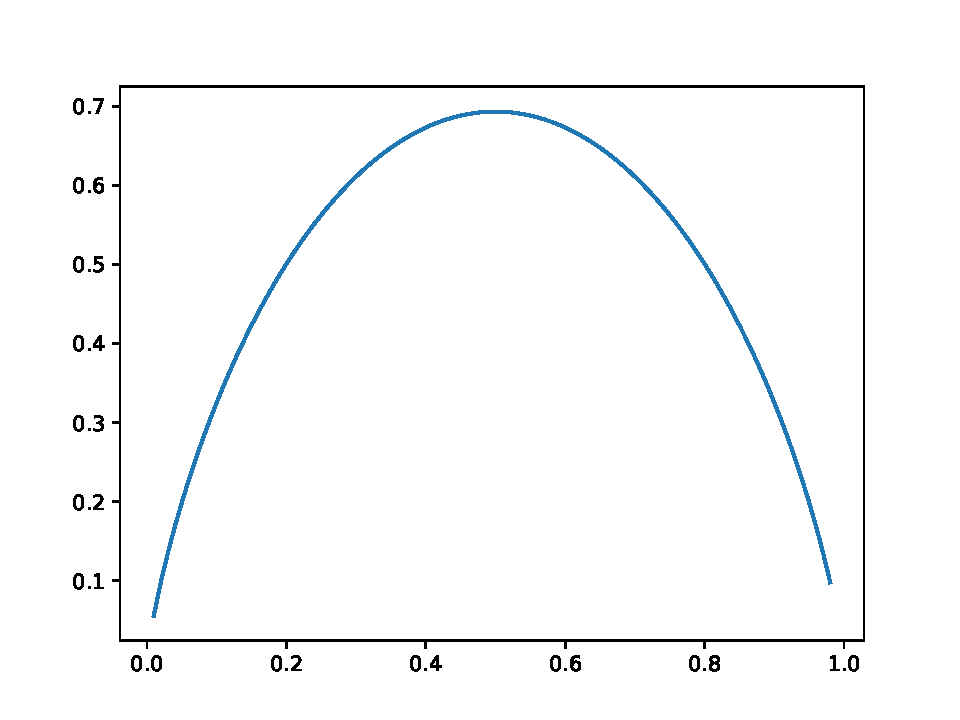
\includegraphics[width=0.45\textwidth]{images/H(X)(coin).pdf}
%     \caption{n=2인 계의 H(X)}
%     \label{H(X, n=2)}
% \end{figure}

그렇다면 계의 확률분포에 대해서 기댓값이 주어진 경우는 어떻게 되는가? 확률분포에 대해서 가장 대중적으로 얻는 값은 기댓값과 표준편차이다. 기댓값이 주어진 경우부터 살펴보자. 사건 $i$에 대응하는 확률변수의 값이 $x_{i}$라고 하자. 또, 주어진 기댓값을 $\mu$라고 한다면 제약조건은 다음과 같다.
\begin{equation}
    \sum_{i} x_{i}p_{i} = \mu
    \label{Constraint2}
\end{equation}

조건 \ref{Constraint1}과 \ref{Constraint2}를 엔트로피에 적용하여 새로운 목적함수를 쓰고 라그랑주 승수법을 적용하면 다음과 같다.

\begin{equation}
    L_{2} = -\sum_{i} p_{i} \ln{p_{i}} - \lambda_{1} ( \sum_{i} p_{i} - 1) - \lambda_{2} (\sum_{i} p_{i}x_{i} - \mu)
    \label{L_II}
\end{equation}

\begin{equation}
    \frac{\partial L_{1}}{\partial p_{i}} = 0:~ -\ln{p_{i}} - 1 - \lambda_{1} - \lambda_{2} x_{i} = 0
    \label{Lagrange_II}
\end{equation}

식 \ref{Lagrange_II}을 정리하면
\begin{equation}
    p_{i} = \exp{(-1-\lambda_{1} - \lambda_{2} x_{i})} = C \exp{(-\lambda_{2} x_{i})}
    \label{p_i(Lagrange_II)}
\end{equation}

의 확률분포를 얻을 수 있다. 이 경우에 $\lambda_{2} \neq 0$이므로 사건 $i$의 확률은 그때의 확률변수 값 $x_{i}$에 대하여 지수함수적으로 비례하고 볼츠만 분포 (Boltzmann Distribution) 이다. 연속 분포에 대해서 제약 조건에 대한 $\lambda_{2}$와 $C$, $\mu$를 구해보면 $C = \lambda_{2} = 1/\mu$임을 알 수 있다 (단, 정의역은 $x>0$으로 제한하였다). 하지만 이산 분포에 대해서는 다르며 $x=1, ~2, ~\cdots, ~n$인 경우를 생각하자.
\begin{equation}
    C(e^{-\lambda}+e^{-2\lambda} + \cdots + e^{-n\lambda}) = 1, ~ \frac{1}{C} = \frac{e^{-\lambda}(1-e^{-n\lambda})}{1-e^{\lambda}}
    \label{C_II}
\end{equation}
\begin{equation}
    C(e^{-\lambda}+2e^{-2\lambda} + \cdots + ne^{-n\lambda}) = \mu
    \label{mu_II}
\end{equation}

식 \ref{C_II}, \ref{mu_II}를 연립하면 다음과 같은 관계식을 얻을 수 있다.
\begin{equation}
    \mu = \frac{1}{1-e^{-\lambda}} - \frac{ne^{-n\lambda}}{1-e^{-n\lambda}}
    \label{mu, n, lambda relation_II}
\end{equation}
이를 풀면 $\mu, n$에 대한 알맞는 $\lambda$를 구할 수 있다. 물리적으로도 기체의 속도 분포를 유도할 때 계의 전체 입자수와 총 에너지가 제한되어 있으며 이는 위의 제약 조건 \ref{Constraint2}와 같다.

% 이산 분포에 대해서는 $\lambda_{2}$를 구할 수 없으며 연속일 때를 가정하겠다. 단, 가능한 Domain은 $x_{i} > 0$이며 이후 시뮬레이션에서는 이를 1, 2, \cdots, 100으로 제한할 것이며 $\lambda_{2} > 0$이어야 하고 연속 가정은 $x$에 대응하는 확률밀도함수를 $p(x)$로 두어 푼다는 의미이다.
% \begin{equation}
%     \int_{0}^{\infty}{C \exp{-\lambda_{2} x} dx} = 1, ~C = \lambda_{2}
% \end{equation}

% \begin{equation}
%     \int_{0}^{\infty}{x C \exp{\lambda_{2} x}dx} = \mu, ~ \mu = 1/\lambda_{2}
% \end{equation}

% 즉, 구하는 분포는 볼츠만 분포와 같은 아이디어를 쓰며 다음과 같다.
% \begin{equation}
%     p(x) = \frac{1}{\mu} \exp{(-\frac{x}{\mu})},~p_i = \frac{1}{\mu} \exp{(-\frac{x_{i}}{\mu})}
%     \label{p_II}
% \end{equation}


통계학적으로 분석을 할 때는 기댓값 뿐만이 아니라 표준편차도 중요하다. 표준편차가 $\sigma$로 주어진 경우를 살펴보자.
\begin{equation}
    \sum_{i} p_{i}x_{i}^{2} - \mu^{2} = \sigma^{2}
    \label{Constraint3}
\end{equation}
이 경우의 목적함수는 다음과 같다.

\begin{equation}
    L_{3} = -\sum_{i} p_{i} \ln{p_{i}} - \lambda_{1} ( \sum_{i} p_{i} - 1) - \lambda_{2} (\sum_{i} p_{i}x_{i} - \mu) - \lambda_{3}(\sum_{i} p_{i}x_{i}^{2} - \mu^{2} - \sigma^{2})
    \label{L_III}
\end{equation}
라그랑주 승수법을 적용하면
\begin{equation}
    \frac{{\partial L_{3}}}{\partial p_{i}} = 0:~ -\ln{p_{i}} - 1 - \lambda_{1} - \lambda_{2} x_{i} - \lambda_{3} x_{i}^{2} = 0
    \label{Lagrange_III}
\end{equation}
\begin{equation}
    p_{i} = \exp{(-1-\lambda_{1} - \lambda_{2} x_{i} - \lambda_{3} x_{i}^{2})} = A \exp{(-\lambda_{3} (x_{i} - B)^{2})}
    \label{p_i(Lagrange_III)}
\end{equation}

이는 가우스 분포 (Gaussian Distribution)이다. 역으로 $D_{KL}(P||Q)$를 이용하여 가우스 분포는 주어진 제약 조건 (식 \ref{Constraint3})에서 $H(p)$가 제일 큰 확률분포임을 알 수 있다. 일반적으로 주어진 모수 $\mu,~\sigma$에 대한 확률분포함수는 다음과 같음을 알고 있다.
\begin{equation}
    p(x) = \frac{1}{\sigma\sqrt{2\pi}}\exp{(-\frac{1}{2}(\frac{x-\mu}{\sigma})^{2})}
\end{equation}
하지만 역시나 이산적인 경우에 대해서 계산을 해주어야 하고 $x=1, ~2, ~\cdots, ~n$인 경우를 생각한다.
\begin{equation}
    A e^{-\lambda (1 - B)^{2}} + A e^{-\lambda (2 - B)^{2}} + \cdots + A e^{-\lambda (n - B)^{2}} = 1
\end{equation}
\begin{equation}
    A e^{-\lambda (1 - B)^{2}} + 2A e^{-\lambda (2 - B)^{2}} + \cdots + nA e^{-\lambda (n - B)^{2}} = \mu
\end{equation}
\begin{equation}
    A e^{-\lambda (1 - B)^{2}} + 2^2 A e^{-\lambda (2 - B)^{2}} + \cdots + n^2 A e^{-\lambda (n - B)^{2}} = \mu^2 + \sigma^2
\end{equation}

위 세 식으로부터 $A$, $B$, $\lambda$를 $\mu, ~\sigma$로 나타내는 것이 목표였으나 사실상 불가능하다. 그나마 얻을 수 있는 관계식은 $\lambda$로 편미분하여 정리할 시 얻어지는
\begin{equation}
    \ln{A} = \lambda((B-\mu)^{2}+\sigma^{2}) + (const)
\end{equation}

이지만 이로는 부족하며 정확한 상수는 알 수 없다.

\subsection{시뮬레이션}

결국 문제의 본질은 주어진 제약 조건 하에서 엔트로피 값을 최대화할 수 있는 확률 분포를 찾는 것이며 이는 최적화 문제로 분류할 수 있다. 이러한 최적화 문제를 해결하는데 대표적인 방법으로는 유전적 알고리즘(이하 GA)가 존재한다. 따라서 본 프로젝트에서는 이 방식을 활용하여 수식 유도의 결과와 실제 최적화 결과가 일치하는지 검증해보고자 한다.

먼저, GA에 대해 알아보자. GA는 다윈의 자연선택설에 기반하여 더 적합도가 높은 유전자들이 확률적으로 더 많이 살아남도록 하고 살아남은 우수한 유전자들끼리 서로 조합하여 더 나은 유전자를 가진 다음 세대를 만든다. 그리고 이 과정을 반복함으로써 최종적으로 최적해를 찾는다. GA를 구성하는 단계로는 초기 유전자 생성, 평가, 교차, 돌연변이가 있으며 본 프로젝트에서 차용한 GA의 연산들은 아래와 같다.

\newpage
\textbf{1. 초기 유전자 생성}

먼저, GA를 통해 확률분포를 최적화하는 것이 목표이기 때문에 이를 유전자로 표현해야 한다. 때문에 확률변수 $X$: $x_i = 1, 2, 3, \cdots, 20 ~(n=20)$에 대하여 각각의 확률 $p_i$를 유전자로 잡았다. 즉, 유전자는 $n=20$인 확률 분포가 되는 것이다.
\begin{equation}
    gene = \{ p_i : 1 \leq i \leq 20\}
    \label{gene}
\end{equation}

한 세대는 750개의 유전자로 구성되어 있으며, 초기 유전자의 경우 합이 1이 되는 랜덤한 실수쌍 10개로 생성하였다.\\

\textbf{2. 평가}

우리가 찾고자 하는 확률 분포는 다음 네 가지 조건을 만족해야 한다.
\begin{itemize}
    \item $\sum_i{p_i} = 1$ (조건 I)
    \item $H(X) = -\sum_i{p_i \ln{p_i}}$를 최대화
    \item $\mathbb{E}[X] = \mu_0$ (조건 II)
    \item $\sigma(X) = \sigma_0$ (조건 III)
\end{itemize}

따라서 평가함수는 이러한 제약 조건들을 반영해야 한다. 다만, 첫 번째 제약 조건의 경우 유전자의 생성 단계에서 고려하여 평가함수에는 반영하지 않도록 하였다. 그 결과 최종적으로 짠 평가함수는 식 (\ref{eq:fitness})과 같다.

\begin{equation}
    \label{eq:fitness}
    fitness = w_1 \times e^{H(X)^2} + w_2 \times \frac{1}{1+(\mathbb{E}[X]-\mu_0)^2} + w_3 \times \frac{1}{1+|\sigma(X)-\sigma_0|}
\end{equation}

각 항에 대해 살펴보면, 첫 번째 항은 $H(X)$를 최대화하기 위함이고, 두 번째 항은 $\mathbb{E}[X]=\mu_0$가 되도록 하기 위해 그 차이가 줄어들수록 값이 커지게 하였고, 세 번째 항은 $\sigma(X)=\sigma_0$는 두 번째 항과 마찬가지 원리로 참값과 가깝게 되도록 한 것이다. 다만, 표준편차의 경우 애초에 그 값과 멀리 떨어진 값에서 출발한 경우가 많아 0으로 수렴할 여지가 다분하여 좀 더 차이가 클 때 적게 반영되도록 절댓값으로 잡게 되었다. 또한, 제약조건이 필요없는 경우 해당 제약조건의 가중치($w_i$)를 0으로 잡아 이가 반영되지 않도록 하였다.\\

\textbf{3. 교차 \& 돌연변이}

새로운 유전자를 생성하는 단계로, 기존의 있던 유전자들을 적합도에 비례하는 확률로 선택하여 해당 유전자끼리 조합하여 다음 유전자를 만들게 된다. 이때, 실제 유전자의 교차 과정을 모방하여 한 지점을 기준으로 그 앞은 부모 1의 유전자, 그 뒤는 부모 2의 유전자를 따르도록 하였다. 또한, 수렴 직전의 상황에서도 더 좋은 유전자가 잘 선택되게 하기 위하여 선택압을 4배로 맞추어, 가장 안 좋은 해와 좋은 해가 선택될 확률이 4배가 되도록 하였다.
교차 이후 유전적 다양성을 확보하기 위하여 일정 확률로 4개 이하의 $i$를 선택하여 각 $p_i$가 $\pm 50\%$의 범위 내에서 변하도록 하였다. 그리고 최종적으로 조건 Ⅰ을 만족시키기 위하여 전체 확률 합이 1이 되도록 비례배분하게 된다.

이 과정을 수식적으로 표현하면 아래와 같다. 부모 유전자 $gene_1$과 $gene_2$를 룰렛 알고리즘을 통해 선택하여 자식 유전자 $gene'$을 만든다고 할 때, $k$번째를 기준으로 교차 연산을 거치면 

\begin{equation*}
    p'_{i, 0} = \begin{cases}
        p_{1, i} & \text{if $\; 0 \leq i \leq k$}\\
        p_{2, i} & \text{if $\; k < i < 20$}
    \end{cases}
\end{equation*}

과 같이 된다. 그리고 변이를 받을 대상의 인덱스를 모은 집합을 $S$라 둘 때, 각 $p'_{i, 0} (i \in S)$에게 $w_i (-0.5 \leq w_i \leq 0.5)$만큼의 변이를 주게 된다면 유전자는 다시 아래와 같이 바뀌게 된다.

\begin{equation*}
    p'_i = \begin{cases}
        (1+w_i) p'_{i, 0} & \text{if $i \in S$}\\
        p'_{i, 0} & \text{else}
    \end{cases}
\end{equation*}

그리고 이렇게 생기게 된 유전자들을 최종적으로 합이 1이 되도록 하기 위하여 합으로 나눠주게 되면 새로운 자식 세대 유전자가 된다. % 연구 과정
	\section{결과 및 결론}

유전 알고리즘을 돌려본 결과, 아래의 그림과 같이 유전 알고리즘이 잘 수렴하였음을 확인할 수 있었으며, 그 결과의 분포 역시 시각화 가능하였다. 이를 통하여 유전 알고리즘의 결과가 실제 계산으로 도출된 결과와 얼마나 유사한 지를 정성적으로 확인 가능하다. 그리고 유전 알고리즘을 작동시키는 과정에서 선택압을 적절히 조절함으로써 해의 수렴성을 높일 수 있다는 사실도 알 수 있었다.

또한, 자체 제작한 평가함수를 이용한 유전 알고리즘의 결과가 KL 지표 상으로도 수렴하고 있음을 확인해볼 수 있는데, 이는 유전 알고리즘에 사용된 평가함수가 정확하였다는 것을 시사한다. 그리고 KL 값 자체가 0으로 수렴하였기 때문에 유전 알고리즘으로 도출된 분포가 통계적으로 실제 수식적으로 유도된 분포와 거의 같다는 것을 정량적으로도 확인해볼 수 있었다. 

다만, 아래의 (Fig. \ref{fig:normal fitness}.)에서는 다른 분포들의 시뮬레이션과는 다르게 KL의 수렴 그래프를 싣지 못하였는데, 이는 앞선 언급했듯이 정규분포의 식은 이산적인 상황에서 유도하지 못하였기 때문이다. 그러나 이 상황에서 역시 적합도 값은 잘 수렴한다는 사실을 알 수 있었다. 그리고 대안으로 같은 평균과 표주편차 값을 갖지만 $(-\infty, \infty)$를 정의역으로 갖는 실제 연속적인 정규 분포와의 대조해보았는데, 그래프의 개형이 거의 유사하다는 것을 알 수 있었다.

결론적으로 본 연구를 통해 정보 엔트로피의 최대화에 다양한 제약 조건을 입히는 것만으로도 우리가 잘 아는 균등 분포, 볼츠만 분포, 그리고 정규 분포가 잘 유도됨을 보일 수 있었다. 특히, 이 과정에서 라그랑주 승수법을 활용하여 다변수 함수의 최솟값을 찾을 수 있었으며, 유전 알고리즘을 통해 이가 실험적으로 검증해볼 수 있었다.

\pagebreak
\begin{figure}[!htb]
    \centering
    \begin{minipage}{.5\textwidth}
        \centering
        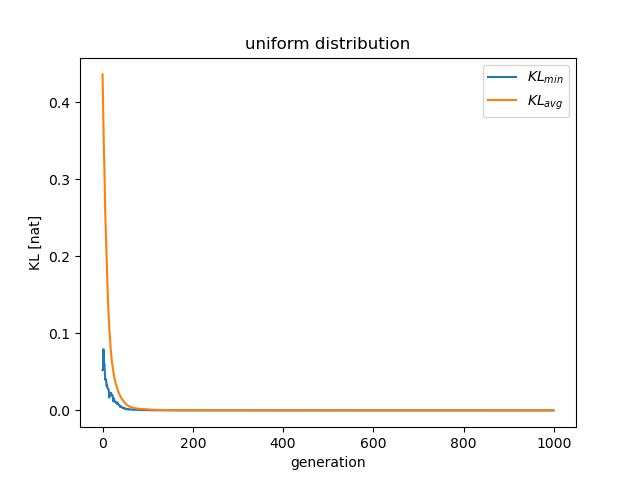
\includegraphics[width=\linewidth, height=0.63\linewidth]{images/uniform convergence KL.png}
        \caption{균등 분포의 KL 수렴 양상}
        \label{fig:uniform KL}
    \end{minipage}%
    \begin{minipage}{0.5\textwidth}
        \centering
        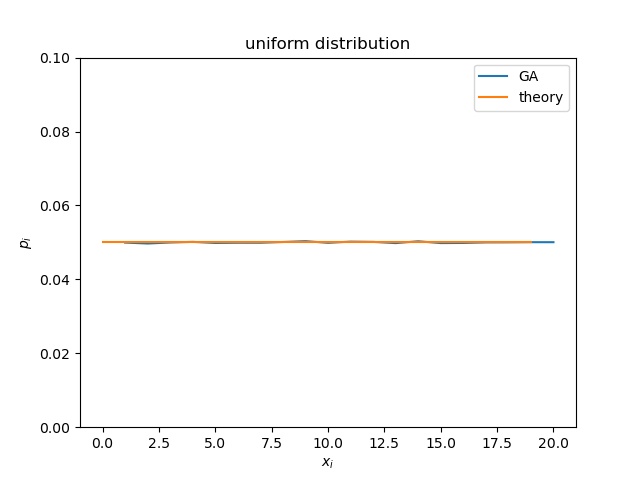
\includegraphics[width=\linewidth, height=0.63\linewidth]{images/uniform result.png}
        \caption{균등 분포의 수렴 결과}
        \label{fig:prob1_6_1}
    \end{minipage}
\end{figure}
\begin{figure}[!htb]
    \centering
    \begin{minipage}{.5\textwidth}
        \centering
        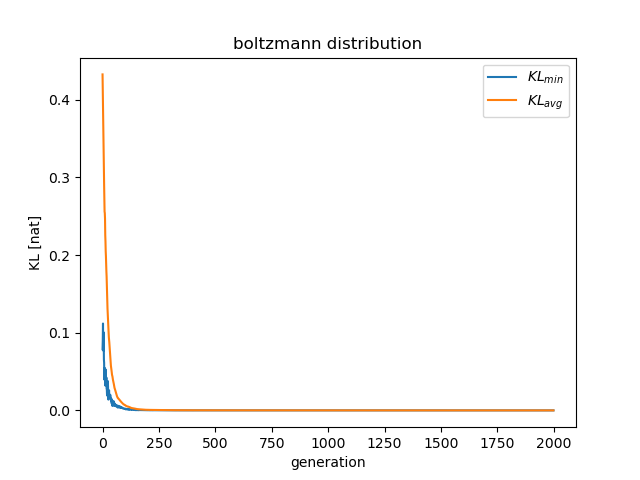
\includegraphics[width=\linewidth, height=0.63\linewidth]{images/boltzmann convergence KL.png}
        \caption{볼츠만 분포의 KL 수렴 양상}
        \label{fig:prob1_6_2}
    \end{minipage}%
    \begin{minipage}{0.5\textwidth}
        \centering
        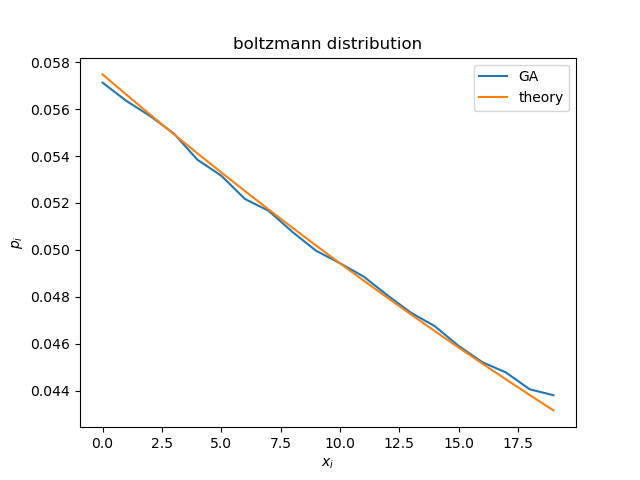
\includegraphics[width=\linewidth, height=0.63\linewidth]{images/boltzmann result.png}
        \caption{볼츠만 분포의 수렴 결과}
        \label{fig:prob1_6_1}
    \end{minipage}
\end{figure}
\begin{figure}[!htb]
    \centering
    \begin{minipage}{.5\textwidth}
        \centering
        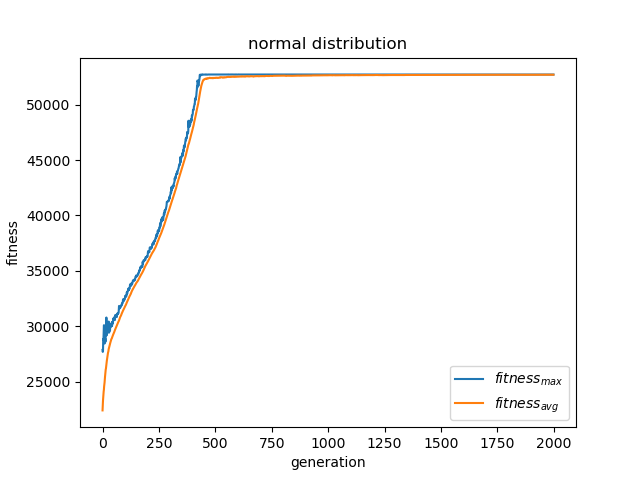
\includegraphics[width=\linewidth, height=0.63\linewidth]{images/normal convergence fitness.png}
        \caption{정규 분포의 적합도 수렴 양상}
        \label{fig:normal fitness}
    \end{minipage}%
    \begin{minipage}{0.5\textwidth}
        \centering
        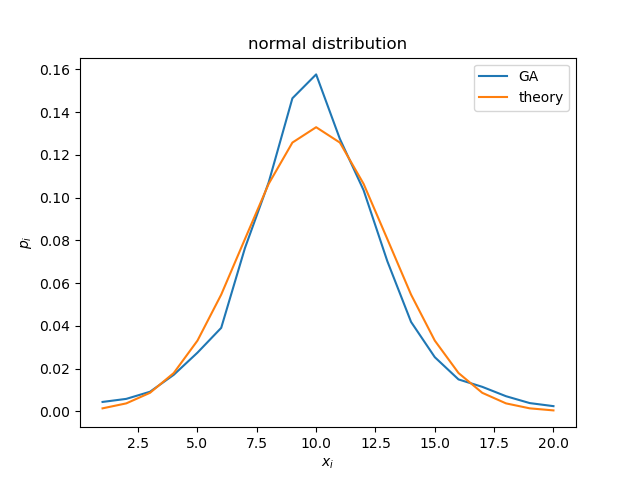
\includegraphics[width=\linewidth, height=0.63\linewidth]{images/normal result.png}
        \caption{정규 분포의 수렴 결과}
        \label{fig:normal result}
    \end{minipage}
\end{figure} % 결과 및 토의
	% \section{결론}
%\section{Conclusion}


 % 결론
	% \section{추후 연구}
%\section{Further research}

\subsection{제목}

내용 % 추후 연구
	% \section{부록}
%\section{Appendix}
 % 부록
        \section{소감}

\begin{itemize}
    \item[] \textbf{김희윤}: 이번에 정보 엔트로피라는 개념을 처음 접하게 되었다. 정보 이론에서 중요한 개념인 정보 엔트로피의 정의와 그 활용에 대하여 배울 수 있었다. 기존의 거시적이고 확정적인 상황과 다르게 불확실한 상태에 대하여 어떤 식으로 정보를 도출해 내고 계산하는지 알 수 있게 되었다. 유전 알고리즘을 적용 시켜 확률을 계산하는 등 다양한 방법으로 최대 정보 엔트로피를 계산하는 과정을 알게 되었다.
    
    
    \item[] \textbf{남도현}: 정보 엔트로피라는 개념은 이전에도 알고 있었으나 이번 기회를 통해 심도있게 다루고 공부해보아서 유익했다. 특히, kullback-leibler divergence라는 개념으로 확률 분포 사이의 일종의 '거리'를 정의할 수 있다는 점이 신기하였다. 또, 물리에서 맥스웰-볼츠만 분포를 배울 때는 물리적 관점에서 접근하였는데 그 기저에 깔린 가정만으로도 같은 분포를 얻을 수 있다는 점을 알 수 있게 되었고 물리적으로 정의된 2개의 엔트로피와 정보 엔트로피가 일맥 상통한다는 점도 알게 되었다. 여러모로 깨달은 점이 많으며 굉장히 흥미로웠고 앞으로도 볼 일이 자주 있을 것 같다.
    
    \item[] \textbf{배요한}: 이번 프로젝트를 통하여 정보 엔트로피라는 개념을 알게 되었는데, 이를 최대화시키는 과정에서 평균을 설정하거나 표준편차를 설정하는 등의 제약 조건 추가만 하였음에도 우리가 잘 아는 분포가 유도될 수 있다는 것이 흥미로웠다. 또한, 유전 알고리즘을 직접 해보는 과정에서 수렴이 잘 되지 않는 상황이 발생하기도 하였는데, 이 과정에서 선택압을 적절히 조절함으로써 해결될 수 있다는 사실도 알 수 있게 되었다. 결론적으로 작지만 되게 흥미로운 연구였으며 다른 제약 조건이 부여되었을 때의 상황도 궁금해졌다.
    
    
\end{itemize}
	
	\bibliography{bibfile} % 참고문헌
	% BibTeX 코드 쉽게 얻어오는 방법 %
	% Google Scholar 에서 검색한 결과에서 `인용'을 클릭한다.
	% BibTeX 코드를 얻고자 한다면, 하단의 `BibTeX' 을 클릭.
	% 코드가 나온다. Ctrl+A, Ctrl+C로 복사, bibfile에 붙여넣기.


\end{document}
